\setlength{\parindent}{0pt}
\chapter{\bf DISCUSSION}

\gls{dna} replication is a highly conserved and regulated temporal process that is essential to genome inheritance. Yet, stochastic effects of \gls{dna} replication might cause mutagenesis contributing to cancer \citep{tomasetti2015variation}. Therefore, an accurate and properly coordinated \gls{dna} replication is needed to prevent errors and to preserve \gls{dna} fidelity which is constantly threatened by both endogenous and exogenous sources during \gls{dna} replication. Considering 70,000 lesions occur in a single cell per day \citep{lindahl2000repair}, \gls{dna} lesions must be removed before the next cell division, to avoid their permanent conversion into mutations. 

On the other hand, \gls{dna} excision repair mechanisms are known to relentlessly coup with \gls{dna} damages that are potential sites of mutations. In deficiencies of mismatch repair and nucleotide excision repair, there are specific mutational signatures associated which contribute to different cancer types \citep{helleday2014mechanisms}. Nucleotide excision repair associated signature 7 displays replication timing differences and replication related strand asymmetry \citep{tomkova2018mutational}. Furthermore, because \gls{erd}s are more reachable relative to \gls{lrd}s, mismatch repair causes a mutation difference between these domains by effectively repairing the mismatches at \gls{erd}s \citep{supek2015differential}. Similarly, \gls{tcr} creates a transcriptional strand asymmetry by repairing adducts only at transcribed strands and leaving the opposite strand untouched \citep{zheng2014transcription}. Even though signature 7 is linked with \gls{dna} replication timing and strand asymmetry \citep{tomkova2018mutational}, the contribution of nucleotide excision repair to mutation differences during replication is still unclear. In this study, we performed Damage-seq and \gls{xrseq} methods on \gls{uv}-irradiated \gls{hela} cells that are synchronized at early and late S phases to quantify \gls{64} and \gls{CPD} damages and their repair events. 

\section{DNA replication elevates local nucleotide excision repair by mediating chromatin opening}

In the first part of the study, we examined the repair rate of nucleotide excision repair at large regions, while replication moves from early S phase to late S phase. To examine the repair rate on replication domains, we mapped damage and repair events to these regions. After calculating the repair rates, we found that \gls{erd}s are repaired more efficiently that \gls{lrd}s. Because \gls{erd}s are usually corresponding to open chromatin sites, they are more reachable for nucleotide excision repair, which in turn, promotes efficient repair. This result suggests that, like mismatch repair \citep{supek2015differential}, nucleotide excision repair creates a mutational difference between \gls{erd}s and \gls{lrd}s by efficiently repairing \gls{erd}s. This phenomenon is less detectable for \gls{64} damages than that of \gls{CPD}s due to fast repair of \gls{64}s.

Then, we examined the differences in repair rates of chromatin states for both \gls{erd}s and \gls{lrd}s. The chromatin states that are associated with close regions are more varying in \gls{erd}s, whereas the chromatin states that are associated with open regions displays same phenomenon in \gls{lrd}s, simply because \gls{erd}s have less close regions, while \gls{lrd}s have less open regions. Expectedly, the active promoters and enhancers are repaired efficiently for both \gls{erd}s and \gls{lrd}s. Moreover, the major difference between phases occurred on close chromatin states. This result indicates that movement of replication elevates the repair rates of close chromatin states by mediating chromatin opening. Lastly, we proposed a simple model to deminstrate the replication effect on repair (Figure \ref{fig:model}).     

\begin{figure}[H]
    \begin{center}
    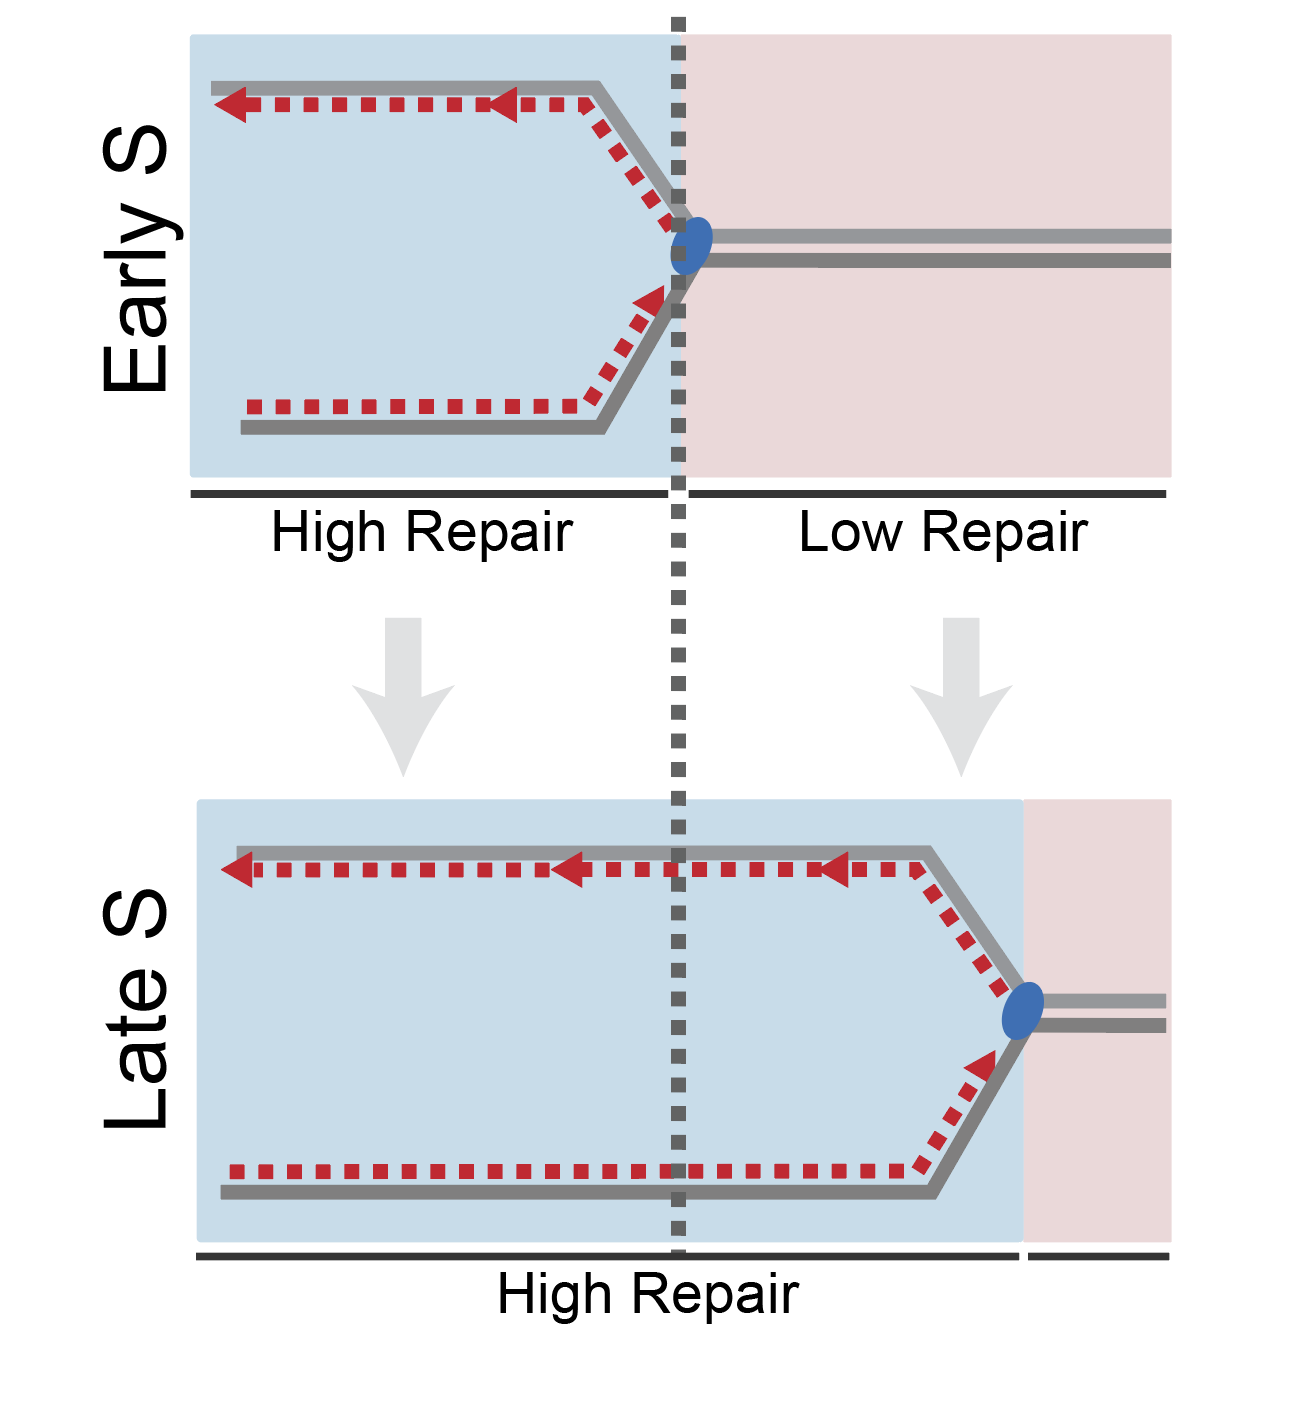
\includegraphics[width=\textwidth]{Chapters/5_discussion/figures/model}
    \caption[Repair preferences of Nucleotide Excision Repair during replication.]{Repair preferences of Nucleotide Excision Repair during replication. During the early S phase, open chromatin regions (blue) which mostly correspond to \gls{erd}s, are repaired better than the condensed regions (red) because excision repair can reach the open chromatin sites more efficiently than it reaches the condensed regions. While replication continues, those condensed regions loosen and become more reachable for excision repair.}
    \label{fig:model}
    \end{center}
    \end{figure}

\section{Mutagenesis, UV-induced DNA damage, and repair display replicational strand asymmetry}

Secondly, we examined a possible replicational strand asymmetry of mutagenesis, \gls{uv}-induced \gls{dna} damage, and repair, respectively. After quantifying the melanoma mutations on initiation zones, we observed a significant mutational strand asymmetry that contains more mutations at lagging strands. Reasoning that this asymmetry around initiation zones should be related to nucleotide excision repair, we mapped damage and repair events on these regions separately. Remarkably, the same asymmetry was detectable for both damage and repair. Then, we simulated Damage-seq and \gls{xrseq} reads to see if the asymmetry is biased by the sequence context and the asymmetry was also detectable for the simulated reads. The results indicates that indeed the strand asymmetry around initiation zones are caused by the sequence context, initially at the level of \gls{uv}-induced damages. Because there are more damages at lagging strands, repair also increases at lagging strands to cope with the damages. Conversely, when we normalized the repair with damage events, repair rates indicates an opposite asymmetry; higher repair rate at leading strands. These results suggest that even though repair events are higher at lagging strands due to high damages, the efficiency of repair elevates at leading strands, which also explains the less mutation counts at leading strands.         
